\section{作业及答案：结构力学基础与技巧班第5次作业及答案（静定桁架）}
\begin{analysisbox}
优先判断零杆，再选择节点法或截面法。节点法适合逐点推进，截面法适合只求少数目标杆件；受拉为正、受压为负的约定要在答案中写清。
\end{analysisbox}
\subsection*{第 1 页转写}
研究生入学考试辅导丛书结构力学（第二版）

图2-139

六、练习题

2-23图2-140所示桁架中零杆的数目为（不包括支座链杆）（

）。（中南大学

2010)

A.6根

B.7根

C.8根

D.9根

2-24计算图2-141所示桁架中1、2杆件的轴力。（重庆大学2010）

图2-140

图2-141

2-25求图2-142所示结构中指定杆件1、2的轴力。（广州大学2012）

2-26求图2-143所示结构中指定杆件1、2的轴力。（广州大学2008）

78
\begin{figure}[H]\centering
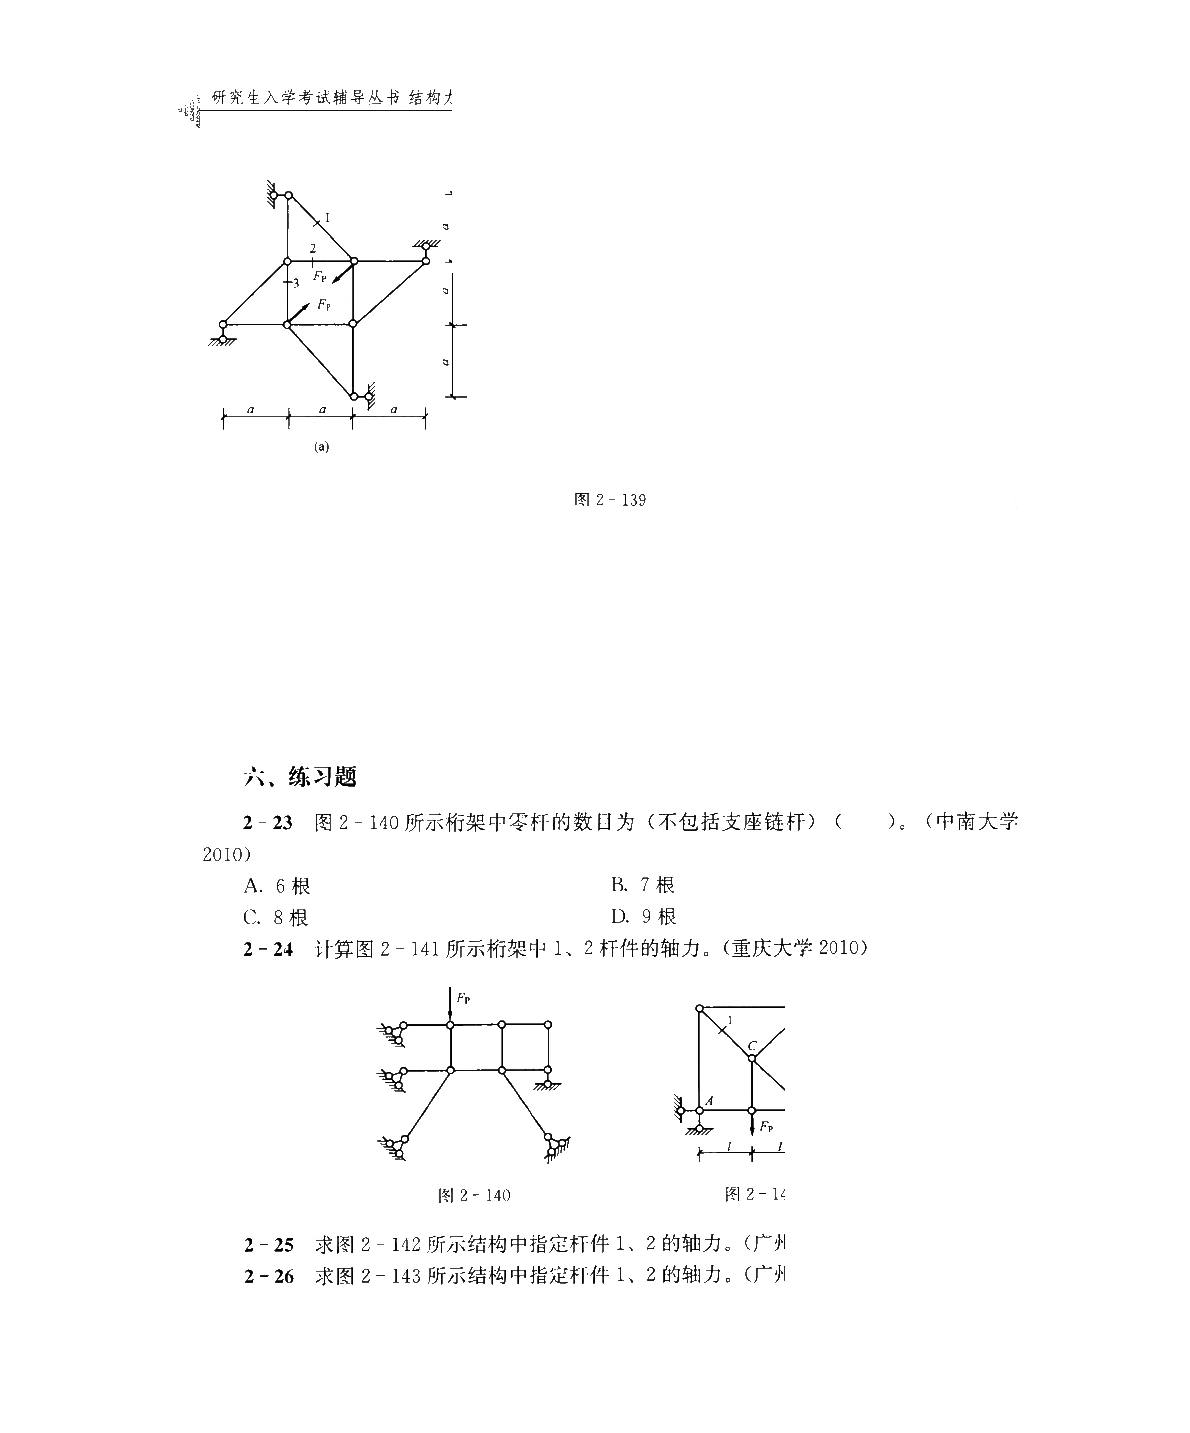
\includegraphics[width=0.92\textwidth]{figures/src08_p001.jpg}
\caption{结构力学基础与技巧班第5次作业及答案（静定桁架） 第 1 页清理图形页}
\end{figure}
\subsection*{第 2 页转写}
50kN

30kN

Fp

图2-142

图2-143

2 - 27

求图2-144所示桁架中1、2杆的轴力。（西南交通大学2008）

2-28作图2-145所示桁架中a、b、c杆轴力。（西南交通大学2010)

Fp

图2-144

图2-145

2 -29

试求图2-146所示桁架中a、b杆件的内力。（东北大学2007)

2-30

求图2-147所示架中a、6杆件的内力。（北京航空航天大学2008）

2d

2d

6x1

图2-146

图2-147

2-31

计算图2-148所示桁架中a、6两杆的轴力。（重庆大学2008)

2-32求图2-149所示桁架中1、2杆件的轴力。（西南交通大学2007）
\begin{figure}[H]\centering
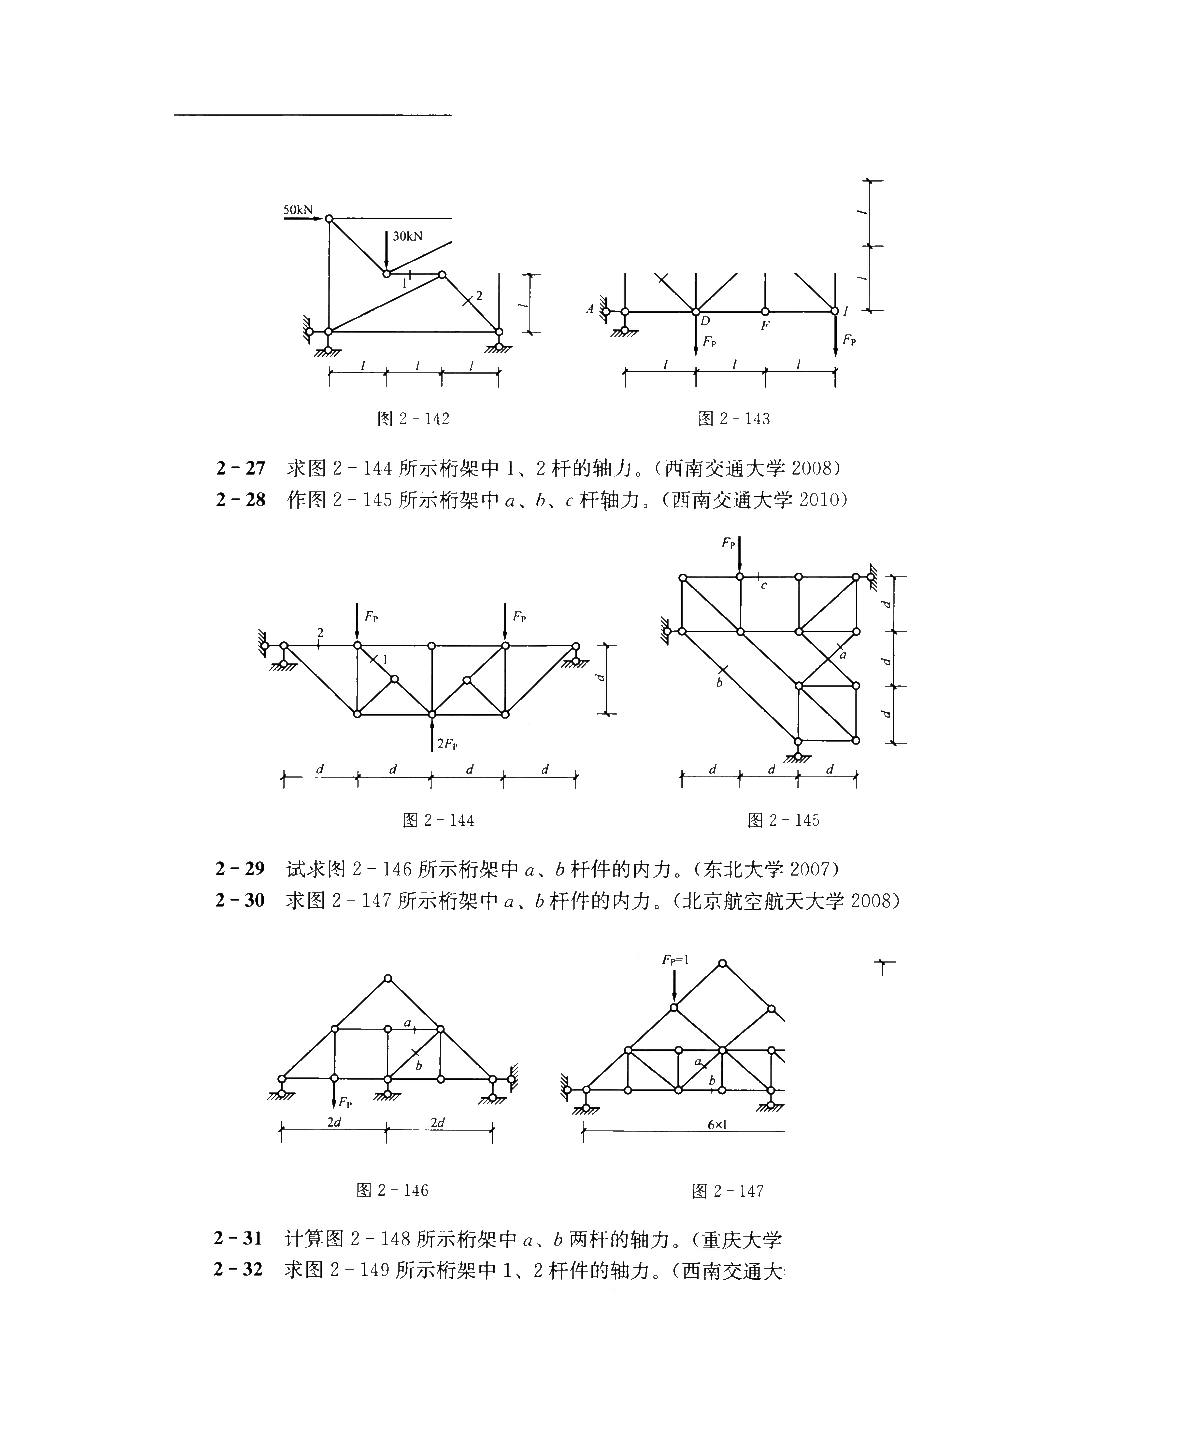
\includegraphics[width=0.92\textwidth]{figures/src08_p002.jpg}
\caption{结构力学基础与技巧班第5次作业及答案（静定桁架） 第 2 页清理图形页}
\end{figure}
\subsection*{第 3 页转写}
研究生入学考试辅导丛书结构力学（第二版）

Fp

Fp

Fp

图2-148

图2-149

七、练习题答案

2-23

C.

2-24

FN=/2Fp/2；Fn2= Fp/2。

2-25

Fnl= 50kN;Fn2=-50/2/3kN。

2-26

Fl=4/2Fp/3；Fn2=2/10Fp/3。

2-27

FN= /2Fp;Fnz=0。

2-28

FNa一/2Fp/2；F\%=/2Fp/2；FN=Fp/2。提示：先求支座反力，再依次取

截面I-I、 - 、 - ，见图2-150。由I-I截面求F（对图中轴列投影方程)，

由I- 截面求FNe，由 - 截面求FN。

2-29Fa= Fp;FN=/2Fp/2。

2-30FNa0；Fb=0.5。提示：集中力右侧和悬臂部分的杆均为零杆，去掉零杆后

结构变为图2-151，由对称性结论可以判断出a杆为零杆，其余零杆也示于图中，6杆的轴

力由结点法求出。

Fp

Fp=1

[Fp

图2-150

图2-151

2-31FN=-/5Fp;Fnb=Fp。

2-32Fn=一/5Fp/2；Fn2=一Fp。提示：先判断出A点连接的两根斜杆为零样

再用结点法或截面法。

80
\begin{figure}[H]\centering
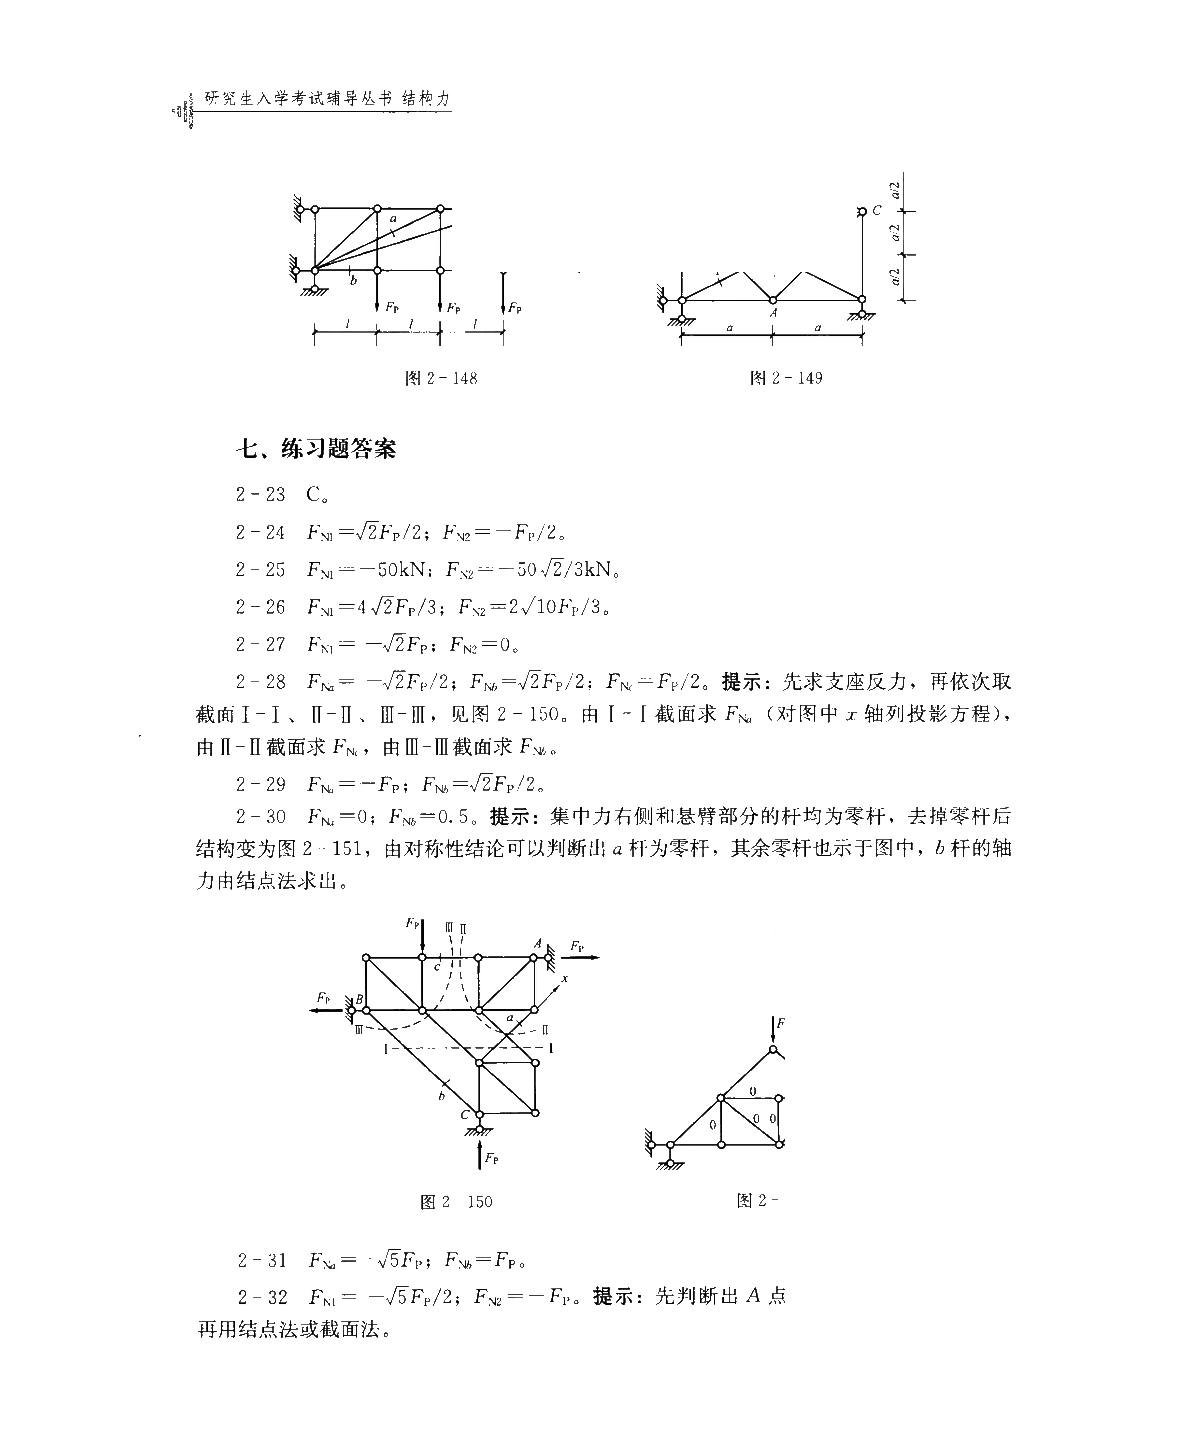
\includegraphics[width=0.92\textwidth]{figures/src08_p003.jpg}
\caption{结构力学基础与技巧班第5次作业及答案（静定桁架） 第 3 页清理图形页}
\end{figure}
